\documentclass[a4paper,12pt]{article}
\usepackage{CJKutf8}
\usepackage{amsthm}
\usepackage{amsmath}
\usepackage{amssymb}
\usepackage{geometry}
\usepackage{tikz}
\usetikzlibrary{chains}
\usepackage{subfigure}
\usepackage{enumerate}

% 边距
\geometry{left=2.0cm,right=2.0cm,top=2.0cm,bottom=3.0cm}

\newtheorem{theorem}{Theorem}
\newtheorem{lemma}[theorem]{Lemma}
\newtheorem{proposition}[theorem]{Proposition}
\newtheorem{corollary}[theorem]{Corollary}
\newtheorem{exercise}{Exercise}
\newtheorem*{solution}{Solution}
\newtheorem{definition}{Definition}
\theoremstyle{definition}

\makeatletter \renewenvironment{proof}[1][Proof] {\par\pushQED{\qed}\normalfont\topsep6\p@\@plus6\p@\relax\trivlist\item[\hskip\labelsep\bfseries#1\@addpunct{.}]\ignorespaces}{\popQED\endtrivlist\@endpefalse} \makeatother
\makeatletter
\renewenvironment{solution}[1][Solution] {\par\pushQED{\qed}\normalfont\topsep6\p@\@plus6\p@\relax\trivlist\item[\hskip\labelsep\bfseries#1\@addpunct{.}]\ignorespaces}{\popQED\endtrivlist\@endpefalse} \makeatother

% 大题
\newenvironment{problems}{\begin{list}{}{\renewcommand{\makelabel}[1]{\textbf{##1}\hfil}}}{\end{list}}

% 小题
\newenvironment{steps}{\begin{list}{}{\renewcommand{\makelabel}[1]{\textbf{##1}\hfil}}}{\end{list}}

% 标题
\title{\small \underline{Mathematical Foundations of Computer Science}\\\Large Project 13}
\author{Log Creative\\\small Student ID: }
\date{\today}

\begin{document}
\maketitle

\noindent\textbf{Warmups}

\begin{problems}
   \item[1] An eccentric collector of $2\times n$ domino tilings pays \$4 for each vertical domino and \$1 for each horizontal domino.  How many tilings are worth exactly \$$m$ by this criterion?  For example, when $m=6$ there are three solutions: 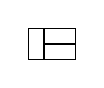
\begin{tikzpicture}
    \draw  (-0.6,0.2) rectangle (-0.4,-0.2);
    \draw  (0,0) rectangle (-0.4,0.2);
    \draw  (0,-0.2) rectangle (-0.4,0);
    \end{tikzpicture}, 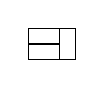
\begin{tikzpicture}
        \draw  (0,0.2) rectangle (0.4,0) node (v1) {};
        \draw  (0,-0.2) rectangle (v1);
        \draw  (0.6,-0.2) rectangle (0.4,0.2);
        \end{tikzpicture}, and 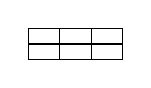
\begin{tikzpicture}
            \draw  (-0.4,0.2) rectangle (0,0) node (v1) {};
            \draw  (-0.4,-0.2) rectangle (v1);
            \draw  (0.4,0) rectangle (0,0.2);
            \draw  (0,-0.2) rectangle (0.4,0) node (v2) {};
            \draw  (0.8,0) rectangle (0.4,0.2);
            \draw  (0.8,-0.2) rectangle (v2);
            \end{tikzpicture}.
    \begin{solution}
        % The problem could be transferred into: How many solutions to $a,b\in\mathbb{N}$,
        % \begin{equation*}
        %     4a + b = m
        % \end{equation*}
        Like what has been done in (7.5), (7.4) could be transferred into      
        \begin{center}
            $T=$\vbox{
                \hbox{\hfill$|$\hfill}
                \vspace*{1pt}
                \hrule
                \vspace*{1pt}
                \hbox{$|$ - \fbox{\vbox to 6.5pt{}} - \vbox{\offinterlineskip\hbox{\fbox{\hbox to 6.5pt{}}}\hbox{\fbox{\hbox to 6.5pt{}}}}}
            } $=\frac{1}{1-z^4-z^2}$
        \end{center}
        whose sequence is
        \begin{equation*}
            \frac{1}{1-z^4-z^2}=\frac{1}{1-z^2-(z^2)^2} \leftrightarrow \langle 0,F_2,0,F_3,0,F_4,\cdots \rangle
        \end{equation*}
        Thus, the number of solutions
        \begin{equation*}
            N = \begin{cases}
                0, &m\text{ is odd,}\\
                F_{\frac{m}{2}+1}, &m\text{ is even}
            \end{cases}
        \end{equation*}
        where $F$ is the Fibonacci number.
    \end{solution}
   \item[2]  Give the generating function and the exponential generating function for the sequence $\langle 2, 5, 13, 35, \cdots \rangle =\langle 2^n+3^n\rangle$ in closed form.
    \begin{solution}
        The generating function for $\langle c^n \rangle $ is $\frac{1}{1-cz}$, according to linearity,
        \begin{equation*}
            \langle 2^n+3^n\rangle \leftrightarrow \frac{1}{1-2z} + \frac{1}{1-3z}
        \end{equation*}
        is its generating function.
        
        The exponential generating function for $\langle c^n \rangle$ is
        \begin{equation*}
            \hat{G}(z) = \sum_{n\geq 0} c^n \frac{z^n}{n!} = \sum_{n\geq 0} \frac{(cz)^n}{n!} = e^{cz}
        \end{equation*}
        Thus, the exponential generating function is
        \begin{equation*}
            \langle 2^n+3^n\rangle \hat{\leftrightarrow} e^{2z} + e^{3z}
        \end{equation*}
    \end{solution}
   \item[3]  What is $\sum_{n\geq 0} H_n/10^n$?
   \begin{solution}
       By (7.57),
       \begin{equation*}
           \langle H_n \rangle \leftrightarrow \frac{1}{1-z}\ln\frac{1}{1-z}
       \end{equation*}
       The convergence radius $R$ of $\langle H_n \rangle $ could be representated as
       \begin{equation*}
           H_n = \sum_{k = 1}^n \frac{1}{k} \leq \sum_{k=1}^n 1 = n \Rightarrow R = \frac{1}{\lim\sup_{n\geq 0} \sqrt[n]{H_n}} = \frac{1}{1} = 1
       \end{equation*}
       (In fact, by recurrence we could get $1 = H_1 = H_0 + 1 \Rightarrow H_0 = 0$, which is satisfiable.)

       Since $\frac{1}{10}<1$ is within the radius,
       \begin{equation*}
           \sum_{n\geq 0} \frac{H_n}{10^n} = \frac{1}{1-\frac{1}{10}}\ln \frac{1}{1-\frac{1}{10}} = \frac{10}{9}\ln \frac{10}{9}
       \end{equation*}
   \end{solution}
   \item[4]  The general expansion theorem for rational functions $P(z)/Q(z)$ is not completely general,  because it restricts the degree of $P$ to be less than the degree of $Q$.  What happens if $P$ has a larger degree than this?
   \begin{solution}
       The problem could be reduced to the scenario where $\deg P < \deg Q$, by applying polynomial division:
       \begin{equation*}
           \frac{P(z)}{Q(z)} = S(z) + \frac{R(z)}{Q(z)}
       \end{equation*}
       where $\deg R< \deg Q$. Since $S(z)$ only influcence finite amount of items (based on its degree), Rational Expansion Theorem can be applied on the second term.
   \end{solution} 
\end{problems}

\noindent\textbf{Basics}

\begin{problems}
    \item[6] Show that the recurrence (7.32) can be solved by the repertoire method, without using generating functions.
    \begin{solution}
        \begin{align*}
            g_0 &= g_1 = 1;\\
            g_n &= g_{n-1} + 2g_{n-2} + (-1)^n, & \text{for }n\geq 2
        \end{align*}
        Consider a general form of
        \begin{align*}
            g_0 &= \alpha;\\
            g_1 &= \beta; \\
            g_n &= g_{n-1} + 2g_{n-2} + (-1)^n\gamma, & \text{for }n\geq 2
        \end{align*}
        has the closed form of
        \begin{equation*}
            g_n = A(n)\alpha + B(n)\beta + C(n)\gamma
        \end{equation*}
        \paragraph{Case 1: $g_n = 2^n$}
        \begin{align}
            \alpha &= 1 \nonumber\\
            \beta &= 2 \nonumber\\
            2^n &= 2^{n-1} + 2\times 2^{n-2} + (-1)^n \gamma \Rightarrow \gamma = 0 \nonumber\\
            g_n &= A(n) + 2B(n) = 2^n \label{eq:1}
        \end{align}
        \paragraph{Case 2: $g_n=(-1)^n$} 
        \begin{align}
            \alpha &= 1  \nonumber\\
            \beta &= -1  \nonumber\\
            (-1)^n &= (-1)^{n-1} + 2(-1)^{n-2} + (-1)^n\gamma \Rightarrow \gamma = 0 \nonumber\\
            g_n &= A(n) - B(n) = (-1)^n  \label{eq:2}
        \end{align}
        \paragraph{Case 3: $g_n = n(-1)^n$}
        \begin{align}
            \alpha &= 0 \nonumber\\
            \beta &= -1  \nonumber\\
            n(-1)^n &= (n-1)(-1)^{n-1} + 2(n-2)(-1)^{n-2} + (-1)^n\gamma  \nonumber\\&\Rightarrow n = -n + 1 + 2(n-2) + \gamma  \nonumber\\ &\gamma = 3 \nonumber\\
            g_n &= - B(n)  + 3C(n)= n(-1)^n \label{eq:3} 
        \end{align}
        Combining Eq. \eqref{eq:1} -- \eqref{eq:3}, the solution is
        \begin{align*}
            A(n) &= \frac{2^n + 2(-1)^n}{3}\\
            B(n) &= \frac{2^n - (-1)^n}{3}\\
            C(n) &= \frac{n(-1)^n}{3} + \frac{2^n-(-1)^n}{9}
        \end{align*}
        So plug in $\alpha = 1,\beta = 1, \gamma = 1$, the closed form is found:
        \begin{equation*}
            g_n = \frac{7}{9}2^n + \left(\frac{1}{3}n + \frac{2}{9}\right)(-1)^n
        \end{equation*}
    \end{solution} 
    \item[7]  Solve the recurrence 
    \begin{align*}
        g_0&=1\\
        g_n&=g_{n-1}+2g_{n-2}+\cdots+ng_0,\quad \text{for }n > 0
    \end{align*}
    \begin{solution}
        The recurrence can be representated by the single equation
        \begin{equation*}
            g_n = \sum_{i=0}^{n-1} (n-i)g_i + [n=0]
        \end{equation*}
        Write down $G(z) =\sum_{n} g_n z^n$,
        \begin{align*}
            G(z) = \sum_{n} g_n z^n &= \sum_n \sum_{i=0}^{n-1} (n-i)g_iz^n + \sum_n [n=0] z^n\\
            &= 1 + \sum_n \sum_{i=1}^n ig_{n-i}z^n\\
            &= 1 + \sum_{i=1}^\infty \sum_n ig_{n-i}z^n\\
            &= 1 + \sum_{i=1}^\infty \sum_n ig_nz^{n+i}\\
            &= 1 + \sum_{i=1}^\infty iz^i\sum_n g_nz^n\\
            &= 1 + \sum_{i=1}^{\infty} iz^{i}G(z)\\
            &= 1 + \frac{z}{(1-z)^2}G(z)\\
            G(z) &= \frac{1-2z+z^2}{1-3z+z^2} \\
            &= 1 + \frac{z}{1-3z+z^2} \\
            &= 1+ \frac{z}{(1-\beta_1 z)(1-\beta_2 z)}
        \end{align*}
        Theorem gives that
        \begin{equation*}
            g_n = [n=0] + a_1 \beta_1^n + a_2 \beta_2^n
        \end{equation*}
        where
        \begin{equation*}
            a_1 = \frac{-\beta_1 \frac{1}{\beta_1}}{-3+2\frac{1}{\beta_1}} = \frac{-\beta_1}{-3\beta_1+2} = -\frac{1}{\sqrt{5}}
        \end{equation*}
        and 
        \begin{equation*}
            a_2 = \frac{-\beta_2 \frac{1}{\beta_2}}{-3+2\frac{1}{\beta_2}} = \frac{-\beta_2}{-3\beta_2+2}= \frac{1}{\sqrt{5}}
        \end{equation*}
        Thus,
        \begin{align*}
            g_n &= [n=0] + \frac{\beta_2^n-\beta_1^n}{\sqrt[]{5}}
        \end{align*}
        where $\beta_1=\frac{3+\sqrt{5}}{2},\beta_2=\frac{3-\sqrt{5}}{2}$.
        Notice that $\beta_1 = \hat{\Phi}^2,\beta_2 = \Phi^2$, thus,
        \begin{align*}
            g_n &= [n=0] +\frac{\Phi^{2n}-\hat{\Phi}^{2n}}{\sqrt[]{5}} \\
            &= [n=0] + F_{2n}
        \end{align*}
        where $F_n=\frac{\Phi^{n}-\hat{\Phi}^n}{\sqrt{5}}$ is the Fibonacci number.
    \end{solution}
\end{problems}

\end{document}
